\section{GraphTXD Klassenreferenz}
\label{classGraphTXD}\index{GraphTXD@{GraphTXD}}
Klassendiagramm für GraphTXD::\begin{figure}[H]
\begin{center}
\leavevmode
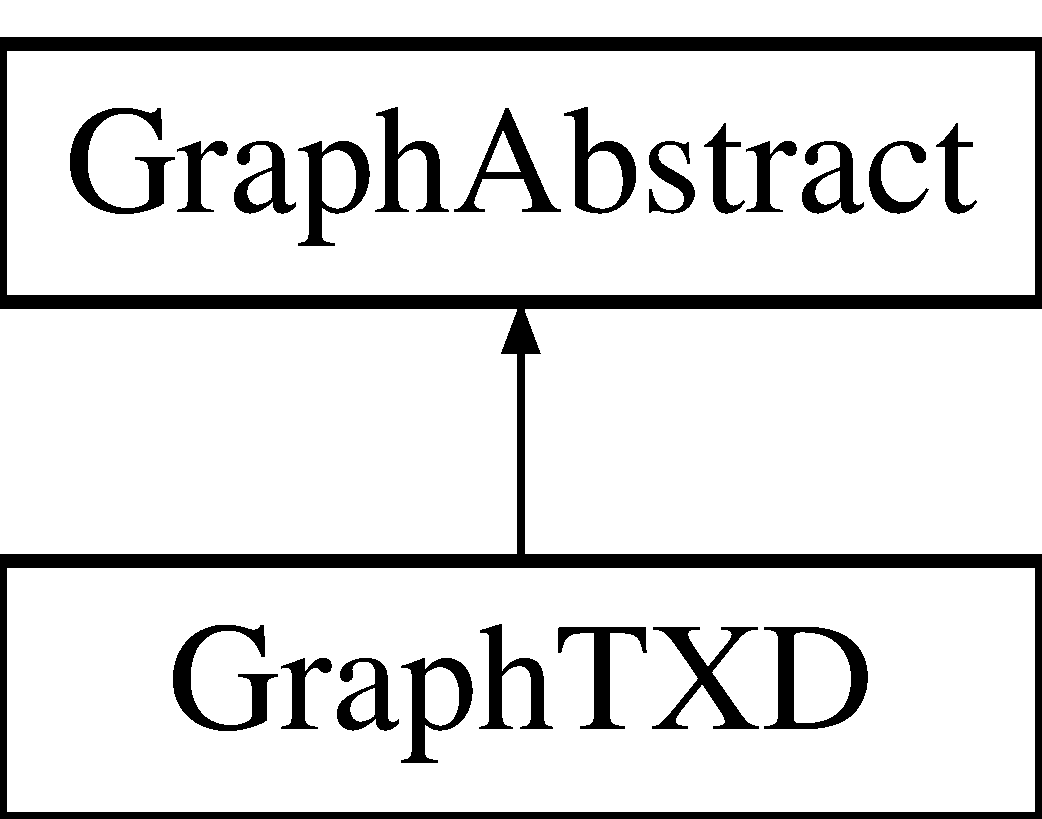
\includegraphics[height=2cm]{classGraphTXD}
\end{center}
\end{figure}
\subsection*{Öffentliche Methoden}
\begin{CompactItemize}
\item 
{\bf GraphTXD} (\$graphId)
\end{CompactItemize}


\subsection{Ausführliche Beschreibung}


Definiert in Zeile 11 der Datei class.GraphTXD.php.

\subsection{Dokumentation der Elementfunktionen}
\index{GraphTXD@{GraphTXD}!GraphTXD@{GraphTXD}}
\index{GraphTXD@{GraphTXD}!GraphTXD@{GraphTXD}}
\subsubsection{\setlength{\rightskip}{0pt plus 5cm}GraphTXD.GraphTXD (\$ {\em graphId})}\label{classGraphTXD_9053944ecf9df3dd4608e5913706e916}




Definiert in Zeile 13 der Datei class.GraphTXD.php.

Die Dokumentation für diese Klasse wurde erzeugt aufgrund der Datei:\begin{CompactItemize}
\item 
{\bf class.GraphTXD.php}\end{CompactItemize}
